\documentclass[]{article}

\usepackage{graphicx}
\usepackage{xepersian}


\settextfont{XB Zar}
\setlatintextfont{Linux Libertine}
\setdigitfont{Parsi Digits}

\begin{document}
\title{طرحِ پیشنهادیِ تولید نرم‌افزارِ کتابخوان و کارسازِ کتاب}
\author{
مؤسسهٔ فرهنگی-هنریِ داده‌گسترِ صبحِ روشن\\\\
اصفهان، سه راهِ سیمین، کویِ ولی‌عصر\\ خیابانِ مولانا، خیابانِ سعادت، کوچهٔ شمارهٔ ۹، پلاکِ ۵۴۴\\
کدِ پستی ۸۱۷۴۷۹۸۴۴۷\\\\
رایانامه: 
\texttt{email@dla.ir}\\
شماره تماس: 
}
\date{\today}
\maketitle
‎\newpage
\tableofcontents
\newpage


\section{کتابخانهٔ دیجیتال}
کتابخانهٔ دیجیتال نمونه‌ای از سیستم‌هایِ «بازیابیِ اطلاعات»
\LTRfootnote{Information Retrieval}
است که در آن مجموعه‌ها در قالب‌هایِ دیجیتالی (در مقابلِ چاپ، میکروفرم، و دیگر رسانه‌ها) ذخیره می‌شوند و توسطِ رایانه‌ها قابلِ دسترس هستند. محتویاتِ دیجیتالی به صورتِ محلی، یا از راهِ دور از طریقِ شبکه‌هایِ رایانه‌ای در دسترس می‌باشند.

بازیابیِ اطلاعات به فناوری و دانشِ پیچیدهٔ جست-و-جو و استخراجِ اطلاعات، داده‌ها، فراداده‌ها در انواعِ گوناگونِ منابعِ اطلاعاتی مانندِ بانکِ اسناد، مجموعه‌ای از تصاویر، و وب گفته می‌شود.

\section{تعداد عنوان کتابِ چاپ‌شده در سال در ایران}
با توجه به این که یکی از شاخصه‌هایی که در عینِ بیانِ رشدِ فرهنگیِ کشور، می‌توان از آن به تحولاتِ آتی پی‌برد، تعداد کتاب‌هایِ چاپ شده در سال است.نمودار زیر وضعیتِ ایران را از سال‌هایِ قبل از انقلاب تاکنون نشان می‌دهد. وضعیتِ ایران در میانِ تمامِ کشورهایِ جهانِ سوم بی‌نظیر است و ایران در این زمینه هم‌ردیفِ کشورهایِ پیشرفتهٔ دنیاست. به طوری که در هر هشت دقیقه، یک کتاب در ایران منتشر می‌شود و بنابرآمارها ایران با چاپِ ۶۵ هزار کتاب در سال، پس از کشورهایِ ايالات متحده آمريكا، انگلستان، چين، روسيه، آلمان، اسپانيا، هند، ژاپن، فرانسه در جایگاهِ دهم قرار گرفته است.
\nocite{Doe:2009:Other,
Doe:2009:Misc,
Doe:2009:Booklet}
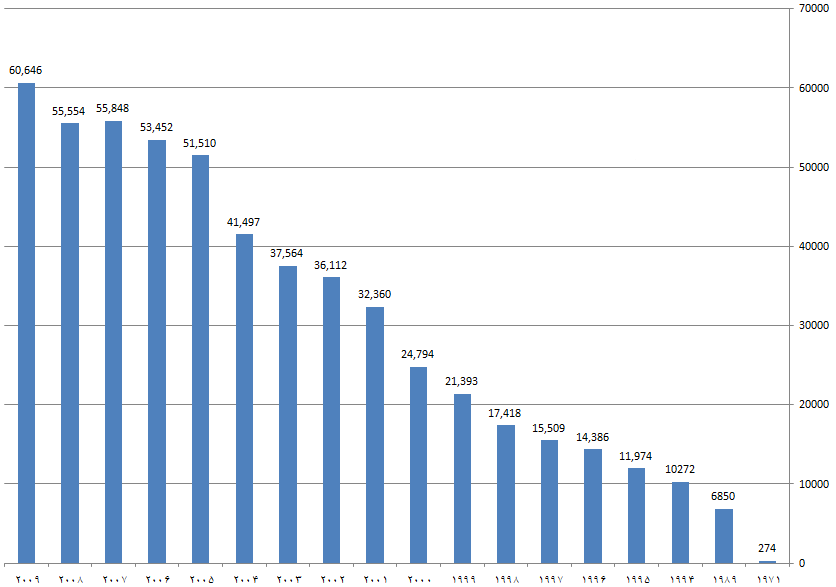
\includegraphics[scale=0.40]{books-of-iran.png}

\section{تعریف طرح}
این طرح به دو مرحله تقسیم می‌شود:
\begin{enumerate}
	\item طراحی و توسعهٔ کتابخانهٔ دیجیتال و نرم‌افزارِ کتابخوان برایِ تلفن‌هایِ هوشمند و رایانه‌هایِ لوحیِ مبتنی بر اندروید.
	\item طراحی و توسعهٔ کارسازِ کتاب و همکاری با مؤسساتِ تحقیقاتی. (طراحیِ بسترِ کتابخانه)
\end{enumerate}
\textbf{گوشزد:}
نباید تصور شود که ارائه‌دهندهٔ این طرح، دو طرحِ مجزا را در دو مرحلهٔ جدا از هم، درون یک طرح گنجانده است. بنده پس از تحقیقاتِ بیشتر در موردِ کتابخانهٔ دیجیتال و روشِ پیاده‌سازیِ نرم‌افزارِ کتابخوان برایِ کتابخانه‌هایِ دیجیتال به این نتیجه رسیدم که بدون داشتنِ یک بسترِ مناسب برایِ کتابخانهٔ دیجیتال، ارائهٔ هر گونه طرحِ عملیاتی برای ساخت نرم‌افزار و کتابخوان برایِ کتابخانه‌هایِ دیجیتال، هزینه‌هایِ زیادی را از نظرِ مالی و زمانی به هدر خواهد داد و نوعی اسراف در به کارگیری نیروها محسوب می‌شود.
\subsection{ویژگی‌هایِ موردِ نظر}
\begin{enumerate}
	\item \textbf{حالتِ مطالعه در شب} 
برایِ سهولتِ مطالعه در شب لازم است که کاربر بتواند نورِ صفحه نمایش را به حداقل مقدار ممکن برساند از این رو می‌توان امکانِ تغییرِ رنگِ پیش‌زمینه به رنگِ سیاه و متن به سفید را فراهم کرد.
	\item \textbf{رنگ قابل تنظیم برای حالت روز/شب}
به علتِ اینکه دو حالتِ شب و روز برایِ مطالعهٔ کاربران در نظر گرفته شده است، بهتر است که کاربر را در انتخابِ رنگِ متون آزاد گذاشت.
	\item پشتیبانی از استاندارد باز و آزاد ای‌پاب\LTRfootnote{ePub}
	\item جست-و-جویِ ساده و پیشرفته در میانِ صفحاتِ کتاب
	\item \textbf{پشتیبانی از پیوند}
در صورتی که پیوندی درونِ کتاب موجود باشد، کاربر می‌تواند با کلیک بر رویِ آن به صفحهٔ مقصدِ پیوند فرستاده شود.
	\item \textbf{پشتیبانی از فهرستِ مطالب\LTRfootnote{TOC: Table of contents}}
در صورتی که کتاب در سطوحِ مختلفی فهرست‌بندی و موضوع‌بندی شده باشد، این نرم‌افزار قابلیتِ حرکت در بینِ سرفصل‌هایِ موردِ نظرِ کاربر را خواهد داشت.
	\item \textbf{همزمان‌سازیِ ابری\LTRfootnote{Cloud Synchronization} برایِ روندِ پیشرفتِ مطالعه}
در صورتی که کاربر چندین رایانهٔ لوحی داشته باشد، برایِ همزمان‌سازیِ روندِ پیشرفتِ مطالعهٔ کتاب در بین رایانه‌هایِ خود می‌تواند از این ویژگی استفاده کند.
	\item \textbf{تغییرِ صفحه با انیمیشن}
برای جذاب ساختن واسط گرافیکی کاربر، جلوه‌های ویژه‌ای برای برگ‌زدن کتاب به صورت عمودی/افقی در نظر گرفته شده است.
	\item \textbf{جست-و-جوی در واژه‌نامه و وب}
کاربر هرگاه با واژه‌ای نا آشنا یا دشوار برخورد کند، می‌تواند واژه را انتخاب کند و توضیحاتِ مربوط به آن را در ویکی‌واژه، ویکی‌پدیا و یا در واژه‌نامهٔ دهخدا جست-و-جو کند.
	\item \textbf{حالتِ تمام صفحه\LTRfootnote{Full Screen}}
کاربر می‌تواند در هنگامِ مطالعهٔ طولانی‌مدت، اندازهٔ صفحهٔ کتابخوان را به حداکثرِ اندازهٔ خود برساند.
	\item \textbf{مرورِ صفحه مبتنی بر مرورگر\LTRfootnote{Browser like scrolling}}
کاربری که با قابلیتِ مرورگرها عادت کرده باشد، می‌تواند به جایِ صفحه‌بندی کتاب، متونِ کتاب را شبیهِ مرورگر پیمایش کند.
	\item \textbf{صفحه‌بندی\LTRfootnote{Pagination}}
کاربرانِ بسیاری عادت دارند به جایِ مرورِ میله‌ای که معمولاً دشوار است، از مرورِ برگه‌ای (ورق‌زدن) برایِ مطالعهٔ کتاب استفاده کنند. نرم‌افزار باید این قابلیت را داشته باشد که متن‌هایِ طولانی را به صفحاتِ کوچکتر متناسب با اندازهٔ صفحهٔ نمایش تبدیل کند.
	\item \textbf{انتخابِ متن و ارسالِ پیامک و رایانامه}
کاربران می‌توانند جملاتِ موردِ نظرِ خود را انتخاب و برایِ دوستانِ خود ارسال کنند.
	\item \textbf{پشتیبانی از سیستمِ توزیعِ نشرِ باز\LTRfootnote{OPDS: Open Publication Distribution System}}
در این روش تمامیِ کتب را می‌توان به صورت توزیع‌شده کاتالوگ کرد و کتب را از راه دور به کاربران ارائه داد. کاربرانی که به اینترنت دسترسی داشته باشند می‌توانند با جست-و-جو در کاتالوگ کتاب‌هایِ موردِ نیازِ خود را بارگیری و مطالعه کنند.
	\item \textbf{نمایشِ پیشرفت به درصد}
نسبتِ تعداد صفحاتِ خوانده شده به کلِ صفحاتِ کتاب را به طور مدام به کاربر نمایش می‌دهد.
	\item \textbf{حذفِ فضاهایِ خالیِ بی‌مصرف}
در صورتی که بین خطوطِ کتاب، فضایِ خالیِ اضافه‌ای وجود داشته باشد، نرم‌افزار به طور خودکار این فضاهایِ خالی را حذف می‌کند.
	\item \textbf{کتاب‌خانهٔ محلی}
نرم‌افزارِ یک کتابخانهٔ محلی برای کتاب‌هایی که بر رویِ دستگاه وجود دارد ایجاد می‌کند تا کاربر راحت‌تر بتواند کتاب‌هایِ خود را مدیریت کند.
	\item کنترلِ میزانِ درخشندگی صفحهٔ نمایش به طورِ مستقل در حالت‌هایِ روز و شب.
	\item قابلیتِ اتصال به شبکه‌هایِ اجتماعیِ کتابخوان و نمایشِ نقدها و بررسی‌هایِ کاربران برایِ هر کتاب
	\item قابلیتِ تنظیمِِ فاصلهٔ بینِ خطوط و اندازهٔ حاشیه‌ها.
	\item قابلیتِ مرورِ خودکارِ صفحات در هنگامِ مطالعه.
	\item قفلِ چرخشِ صفحه.
	\item پشتیبانی از پاورقی در پایانِ صفحات.
	\item بوکمارک و ذخیرهٔ صفحاتِ موردِ علاقهٔ کتاب
	\item نوشتنِ حاشیه برایِ کتاب
	\item تنظیمِ اندازه و نمایِ قلم.
	\item انتخابِ متن و ارسالِ آن‌ها از طریقِ پیامک یا رایانامه
	\item شمارشِ تعداد کاربران از طریقِ ارسالِ پیامک
	\item ارسالِ بازخورد، پیشنهاد، انتقاد و یا سپاسگزاری از طرفِ کاربران
	\item طراحیِ رابطِ برنامه‌نویسیِ نرم‌افزار برایِ پایگاهِ داده‌هایِ کتابخانه و استقرارِ آن رویِ کارسازهایِ رایانشِ ابری، جهتِ اتصالِ کاربران به کتابخانه و دریافتِ کتاب‌هایِ موردِ نیاز، بدونِ نیاز به نصبِ برنامهٔ جداگانه برایِ هر کتاب
\end{enumerate}

\subsection{طراحی و توسعهٔ کارسازِ کتاب}
هر نرم‌افزاری یک ورودی و خروجیِ مشخصی دارند، در مرحلهٔ قبل، نرم‌افزارِ کتابخوان مبتنی بر بسترِ اندروید معرفی شد. اما اینکه این نرم‌افزار کتاب‌ها را از کجا و چگونه بارگیری و نمایش دهد را توسطِ مفهومی به نامِ مخزنِ کتاب یا کارسازِ کتاب دنبال خواهیم کرد. در این سیستم، کتاب‌ها بر اساسِ استانداردِ ای‌پاب بر رویِ مخزنی قرار می‌دهیم که منطبق بر مشخصاتِ اُدی‌پی‌اس است. در این روش تمامیِ کتاب‌ها بر رویِ کارسازی متمرکز می‌شوند و در نهایت کاتالوگی از آن‌ها برای مصرفِ برنامه‌هایِ کتابخوان ایجاد می‌شود. کاربران، با اضافه کردنِ نشانیِ مخزنِ کتاب به کتابخوانِ خود می‌توانند به کاتالوگِ کتاب‌ها دسترسی داشته باشند و در میانِ انبوهی از کتاب‌ها، جست-و-جو کرده و کتابِ موردِ نظرِ خود را پیدا و دریافت کنند.

از آن‌جا که مؤسساتِ بسیاری در کارِ تولیدِ محتوا و کتاب هستند، می‌توان راهنمایِ مناسبی برایِ این مؤسساتِ برایِ ساختِ کارسازِ کتاب ایجاد کرد و حتا کارِ پشتیبانیِ تولید کارسازِ و مخزنِ کتابِ مؤسساتِ مختلف را در دست گرفت.
\section{بررسیِ کتابخانه‌هایِ دیجیتالی}
بر رویِ وبِ فارسی، تا به حال تلاش‌هایِ بسیاری برای ارائهٔ محتوایِ دیجیتایز شده انجام شده است و کتابخانه‌هایِ دیجیتالیِ گوناگونی وجود دارد، در این قسمت سعی می‌کنم کاستی‌هایِ کتابخانه‌هایِ موجود را به طور عام بیان کنیم.
\begin{enumerate}
	\item \textbf{عدمِ رعایتِ استانداردها}\\
در اکثرِ کتابخانه‌هایِ دیجیتالیِ موجود در وب، توجهٔ ویژه‌ای به استانداردهایِ باز نشده است. می‌توان به جرئت گفت که عدمِ توجه به چنین موضوعی سرمنشأ اکثر و شاید تمامیِ کاستی‌هایِ دیگرِ این کتابخانه‌ها به شمار می‌رود. در صورتی که نخواهیم با استانداردهایِ باز همراه شویم، متحملِ ضررهایِ بیشماری خواهیم شد، به طوری که مجبوریم سال‌ها تجربیاتِ اندیشمندانِ گوناگون در آن حوزه را نادیده بگیریم و از ابتدا چرخ را اختراع کنیم. شاید بسیاری از سازمان‌های‌ِ کوچک و متوسط
\LTRfootnote{SME}
در ابتدای کار به این فکر می‌کنند که استفاده از استانداردهایِ باز به صرفه نیست و بهتر است که برای افزایشِ سرعتِ تولیدات خود از روش‌هایِ ابتداعی خود برایِ تولیدِ نشریات و محتویاتِ خود استفاده کنند. این طرزِ تفکرِ نادرست از آنجا ناشی می‌شود که در این مؤسسات، تنها هزینه‌هایِ تولید را در نظر می‌گیرند در صورتی که مؤسسه پس از تولید، باید بتواند، محتوایِ خود را نگهداری، پشتیبانی، به روز کند و حتا گاهی پیش می‌آید که مؤسسات تصمیم می‌گیرند بسترهایِ عملیاتیِ خود را مهاجرت دهند، و معمولاً مؤسساتی که بسترهایِ خود را طبقِ استانداردها تعریف نکرده باشند، هنگامِ مهاجرت هزینه‌هایِ بسیار بالایی را متحمل می‌شوند. 

مزایایِ استفاده از استانداردهایِ باز تنها به موارد زیر محدود نمی‌شود، از این رو برایِ مطالعهٔ بیشتر در این زمینه به کتابِ «مقدمه‌ای بر استانداردهایِ باز، دکتر محمد خوانساری، دکتر حمیدرضا ربیعی، مهندس زهرا احمدی، طرحِ ملیِ نرم‌افزارهایِ آزاد/متن‌باز، با هدایتِ علمیِ مرکزِ تحقیقاتیِ فناوریِ اطلاعات و ارتباطاتِ پیشرفتهٔ دانشگاهِ صنعتیِ شریف» رجوع کنید.
	\begin{enumerate}
		\item بالا بردنِ سطحِ کیفیِ محصول
		\item امنیت و اعتبار بالا
		\item هم‌کنش‌پذیری \LTRfootnote{Interoperability} در میانِ بسترهایِ دیگر
		\item عدمِ وابستگی به فروشنده یا فناوریِ خاص
		\item مهاجرتِ آسان با هزینه‌هایِ کم
		\item پشتیبانیِ طولانی-مدت\LTRfootnote{On-going support}
		\item قابلِ دسترس برایِ استفادهٔ عموم
		\item فناوریِ بی‌طرف
	\end{enumerate}
\item \textbf{مبتنی بر رایانشِ ابری نیستند}\\
این کتابخانه‌ها توجهِ ویژه‌ای بر چگونگیِ ارائهٔ خدماتِ خود برایِ مشتریان ندارد. همچنان در فکرِ بازارِ عرضه و تقاضایِ سنتی هستند و به دنبالِ اسم‌هایِ تبلیغاتی مانند «پکِ جامعِ کتابخانهٔ دیجیتال بر روی دی‌وی‌دی و ...» هستند. این‌ها همگی از عدمِ درکِ درستِ مسؤولان از روندِ پیشرفتِ فناوری‌ست. در سال‌هایِ اخیر، مدل‌هایِ کسب-و-کار از حالتِ سنتیِ خرید و فروشِ کالا به سمتِ ارائهٔ خدمات پیش رفته است و یکی از بزرگ‌ترین تحولاتِ عمده در این زمینه، فناوریِ رایانشِ ابری‌ست که معادلاتِ کسب-و-کارِ سنتی را دگرگون کرده است. برایِ مطالعهٔ بیشتر در این زمینه به سلسله مقالاتِ اینجانب در همین زمینه مراجعه کنید.
\item \textbf{داده‌ها قابل حمل نیستند}\\
همهٔ کاربران همیشه به اینترنت دسترسی ندارند، بعضی از آن‌ها هر از گاهی می‌توانند از اینترنت استفاده کنند و بعضی دیگر از رایانه‌هایِ قابلِ حملِ کوچک و بزرگی استفاده می‌کنند که هنوز این کتابخانه‌هایِ دیجیتالی برای استفاده در این گونه دستگاه‌ها راهِ حلِ مناسبی را ارائه نکرده‌اند.
\item \textbf{هم‌کنش‌پذیر نیستند}\\
کتابخانه‌ای که نتواند با دیگر خدماتِ وبی ارتباط برقرار کند، مسلماً کاربرانِ کم‌تری را جذب خواهد کرد. آن‌ها معمولاً تافته‌ای جدابافته از دیگر خدماتِ رایانه‌ایِ رویِ وب هستند و به ارتباط با دیگر خدماتِ موجود فکر نمی‌کنند. یا حداقل رابطِ برنامه‌نویسیِ برنامهٔ کاربردی را برایِ برنامه‌نویسان پیاده نکرده‌اند.
\item \textbf{عدمِ توجه به نیازهایِ کاربران}\\
یکی از اصولِ مهم در طراحیِ نرم‌افزار، به خصوص در زمینهٔ کتابخانهٔ دیجیتال، بررسیِ نیازهایِ کاربران است. این که ما بتوانیم محتوایِ عظیمی را به کاربران ارائه دهیم ولی سهولت استفاده برای کاربران را در نظر نگیریم، باعث می‌شود که کاربر نتواند آن گونه که باید از کتابخانه استفاده کند. برایِ مثال، پیشنهاد می‌شود که مرکزِ تحقیقاتِ رایانه‌ایِ قائمیه، به جایِ ارائهٔ هر کتاب در یک نرم‌افزار (که حقیقتاً این موضوع مسئلهٔ آزاردهنده‌ای برایِ کاربرانِ نهایی‌ست) نرم‌افزاری تهیه کند که کاربرانِ کتاب‌هایِ موردِ نیازِ خود را یک‌جا دریافت و مطالعه کنند.

\end{enumerate}

%\subsubsection{فهرستِ کتابخانه‌هایِ موجود}
%\begin{enumerate}
%	\item کتابخانهٔ دیجیتالِ دانشگاهِ پیام‌نور
%	\item 
%\end{enumerate}

\section{طرحِ کسب-و-کار}
\subsection{بررسیِ نیازِ بازار}
به نظر می‌رسد مرکزِ تحقیقاتِ رایانه‌ایِ قائمیهٔ اصفهان اولین مرکزی‌ست که به سمتِ تولید کتابخانهٔ‌ دیجیتال برایِ رایانه‌هایِ قابلِ حمل رفته است. این مرکز، برنامه‌ای مبتنی بر جاوا در نظر گرفته‌اند. پروژهٔ جاوا برایِ نسلِ قبلی تلفن‌هایِ همراه طراحی شده بود در حالی که در نسلِ جدید رایانه‌ایِ قابلِ حمل، مفهومی به نامِ رایانشِ قابلِ حملِ هوشمند مطرح شد که در این رایانه‌ها دیگر بستر و سیستم‌عاملی که برایِ طراحی برنامه‌هایِ کاربردی در نظرگرفته می‌شود، اکثرِ نیازهایِ برنامه‌نویسان را مرتفع می‌کند و معایبِ سیستمِ قدیمیِ جاوا را ندارد. به همین دلیل، مرکزِ تحقیقاتِ رایانه‌ایِ قائمیهٔ اصفهان در نظر دارد تا کتابخانهٔ دیجیتالِ خود را بر رویِ بسترِ جدید گوشی‌هایِ تلفن همراه پیاده کند. از این رو آن‌ها به دنبالِ طراحی و پیاده‌سازی نرم‌افزارِ کتابخوان مبتنی بر اندروید هستند.
\subsection{راهِ حل‌ها}
\subsubsection{تولیدِ محصول بر اساسِ نیاز مشتری}
در این مدل ابتدا سازمان و مؤسسه‌ای که نیاز به چنین محصولی دارد را شناسایی می‌کنیم. در اینجا «مرکزِ تحقیقاتِ رایانه‌ایِ قائمیهٔ اصفهان» سپس برایِ تولیدِ نرم‌افزار موردِ نظرِ آن‌ها اقدام می‌کنیم. این روش طرح زودبازده است ولی نتایج آن نامطلوب است. چرا که معمولاً سازمان‌ِ هدفِ ما حاضر نمی‌شود که بر اساسِ ساختار و قالبِ استانداردی که محصول‌مان را ارائه می‌دهیم فعالیت کند و بنابراین مجبور خواهیم شد که نرم‌افزاری منحصراً بر اساسِ سلایقِ ناکارآمدِ سازمانِ موردِ هدف طراحی کنیم و در پایان این محصول را نمی‌توان به طور گسترده در بازار ارائه کرد. البته می‌توان با گفت-و-گو با سازمان، موردِ نظر، آن‌ها را قانعِ کنیم تا بستر خود را به استانداردهایِ باز مهاجرت دهند.
\subsubsection{تولیدِ محصول بر اساسِ نیازِ کاربر}
در این مدل نیازِ کاربر در اولیت بالاتری نسبت به نیازِ سازمان دارد چرا که فعالیت سازمان‌ها وابسته به کاربرانِ نهایی هستند. ابتدا نیازِ کاربر سنجیده می‌شود و سپس بر اساسِ نیازِ کاربر محصولِ نهایی آماده می‌شود. در این صورت چون از فناوریِ بی‌طرف بهره خواهیم برد، نرم‌افزارِ تولیدی بازارِ بیشتری خواهد داشت.
\subsubsection{ارائهٔ خدمات به جایِ ارائهٔ محصول}
در این روش به جایِ طرحِ کسب-و-کارِ سنتیِ خرید و فروشِ محصول، به سمتِ ارائهٔ خدمات می‌رویم، در این مدل، به جایِ فروش و تحویلِ نرم‌افزارِ تولید شده، نرم‌افزارِ تولیدی را خودِ مؤسسهٔ تولید کنندهٔ نرم‌افزار در دست می‌گیرد و توسطِ راهکارهایِ دیگر، به دیگر سازمان‌ها خدمات ارائه می‌کند. برایِ مثال در موضوعِ کتابخانهٔ دیجیتال، مؤسسه می‌تواند، بستری را برایِ تولید محتوا توسطِ دیگر مؤسسات فراهم کند. \\
\textbf{گوشزد:}
این مدلِ کسب-و-کار را خدمت-بنا-به-درخواست
\LTRfootnote{On-demand Service}
نیز می‌گویند.
\section{مراحلِ زمانیِ اجرایِ طرح}
این بخش کامل نشده و در حالِ تکمیل است ... \\
خلاصه: اجرایِ طرح‌هایِ نرم‌افزاری به روشِ RUP باعث می‌شود که به جایِ این که ماه‌ها بر رویِ تولیدِ نرم‌افزار تمرکز کنیم، سعی می‌کنیم در توالی‌هایِ متعدد چرخهٔ تولیدِ نرم‌افزار را تکرار کنیم. به این صورت که نرم‌افزار در بازه‌هایِ زمانیِ متعدد طراحی و استقرار می‌یابد. در این روش، سعی می‌شود از همان ابتدایِ تولیدِ نرم‌افزار واردِ جریانِ استقرار نرم‌افزار می‌شویم تا کارفرما لحظه به لحظه خروجیِ نرم‌افزار را ببیند و اطمینیانِ بیشتری به روندِ تولیدِ پروژه پیدا کند.
\section{ضرورتِ استفاده از استانداردِ ای‌پاب}
استانداردِ مورد نظر ما برایِ پیاده‌سازیِ کتاب‌ها، ای‌پاب است. این استاندارد
\LTRfootnote{EPUB}
برایِ محتویاتِ بازجاری‌پذیر
\LTRfootnote{Reflowable Contents}
 طراحی شده است به این معنی که دستگاه‌هایِ خوانندهٔ این قالب بتوانند نحوهٔ نمایش متنِ موجود در کتاب را برای صفحهٔ نمایشِ خود بهینه کنند.

به دلیلِ اینکه دستگاهِ هدفِ ما برایِ نمایشِ کتاب‌ها، رایانه‌هایِ لوحی و قابلِ حمل ا‌ست، از این رو باید در نظر داشته باشیم که اندازهٔ صفحهٔ نمایشِ رایانه‌هایِ لوحی از یکدیگر بسیار متفاوتند و این تفاوتِ اندازه در بازار نباید در نمایشِ کتاب‌ها تأثیر بگذارد. در قالبِ ای‌پاب به دلیلِ اینکه متون، بازجریان‌پذیر هستند از این نظر دیگر در نمایشِ متون در دستگاه‌هایی با اندازهٔ صفحه‌نمایش متفاوت مشکلی نخواهیم داشت.

ای‌پاب به دلیلِ اینکه استانداردِ باز و آزادی‌ست در همراه شدن با جامعهٔ جهانی جهتِ تولید، نگهداری، مدیریت و نمایشِ این استاندارد سرعتِ بیشتری به دست خواهیم آورد و نکتهٔ قابلِ توجهِ دیگر این است که استفاده از این استاندارد ما را به پیاده‌سازیِ نرم‌افزارِ کتابخوان برایِ تمامیِ بسترها و سیستم‌عامل‌ها رهنمون می‌کند. از این رو هزینه‌هایِ مرتبط با تولید، نگهداری، استقرارِ کتابخانهٔ دیجیتال را کاهش داده و مؤسسه هر زمان که بخواهد کتابخانهٔ دیجیتالِ خود را بر اساسِ بسترهای دیگر، مثل بسترِ وب پیاده کند، برایِ مهاجرت هزینه‌هایِ کم‌تری را متحمل می‌شود و آسان‌تر می‌تواند نسخهٔ ابریِ کتابخانهٔ خود را پیاده کند.
\subsection{ویژگی‌هایِ استاندارد ای‌پاب}
\begin{enumerate}
	\item آزاد و باز
	\item اندازهٔ متون قابلِ تغییر و بازجریان‌پذیر هستند (بسته‌بندیِ متون)
	\item تصاویر شطرنجی و برداریِ درونی
	\item فراداده‌هایِ درونی
	\item پشتیبانی از مدیریتِ حقوقِ دیجیتال\LTRfootnote{DRM: Digital Right Management}
	\item قالب‌بندیِ سی‌اس‌اس
	\item استفاده از نواحیِ درون‌خطی و برون‌خطیِ اکس‌ام‌ال، برایِ گسترشِ کاراییِ ای‌پاب
\end{enumerate}

\section{ضرورتِ استفاده از اُ‌دی‌پی‌اس}
%\subsection{طرحِ مشکل/سناریو}
\subsection{خوانندگان چه می‌خواهند؟}
آن‌ها می‌خواهند این توانایی را داشته باشند که کتاب‌هایِ مورد نیاز خود را، در قالب‌هایِ قابلِ استفاده‌ای که می‌توانند استفاده کنند، برایِ بستر مطالعاتیِ انتخابیِ خود، از هر منبعی، پیدا کنند. کاربران به دنبال راهی هستند که کتاب‌هایِ خود را در حداقل زمانِ ممکن بتوانند پیدا کنند. جست-و-جویِ نامِ کتاب در در بینِ وب‌گاه‌ها و کتابخانه‌هایِ عمومیِ متعدد برایِ یافتنِ کتابِ موردِ نظر به عللِ متفاوتی طاقت‌فرساست:
\begin{enumerate}
	\item کاربر برایِ یافتنِ کتابِ موردِ نظرِ خود مجبور است که نامِ کتاب را در کتابخانه‌هایِ متعددی جست-و-جو کند تا آن را پیدا کند.
	\item پس از اینکه کاربر کتاب را پیدا می‌کند احتمالاً باید به عضویتِ آن کتابخانه در آید.
	\item سامانهٔ جست-و-جویِ کتابخانه‌ها متفاوت است و این باعثِ سردرگمیِ کاربران می‌شود.
	\item مراحلِ دریافتِ دریافتِ کتاب در هر کتابخانه متفاوت است و این برایِ کاربران آزاردهنده است.
\end{enumerate}
\subsection{توزیع‌کننده‌هایِ کتاب (ناشران، کتابخانه‌ها، کتابفروشی‌ها) چه می‌خواهند؟}
کتاب‌هایِ بسیاری با اطلاعاتِ توصیفیِ دقیقی، در هرجا که ممکن است، تحتِ شرایطِ مجازِ فروش/استفاده برایِ جست‌-‌و-‌جو موجودند. توزیع‌کننده‌هایِ کتاب به دنبالِ این هستند که به ساده‌ترین شکلِ ممکن، با بهترین مدلِ کسب-و-کار کتاب‌هایِ خود را تحتِ اجازه‌نامه‌هایِ مختلف به کاربران عرضه کنند.
\subsection{نمایِ وبیِ ارتباطِ بینِ کاربران و کتابخانه‌ها بر رویِ وب}
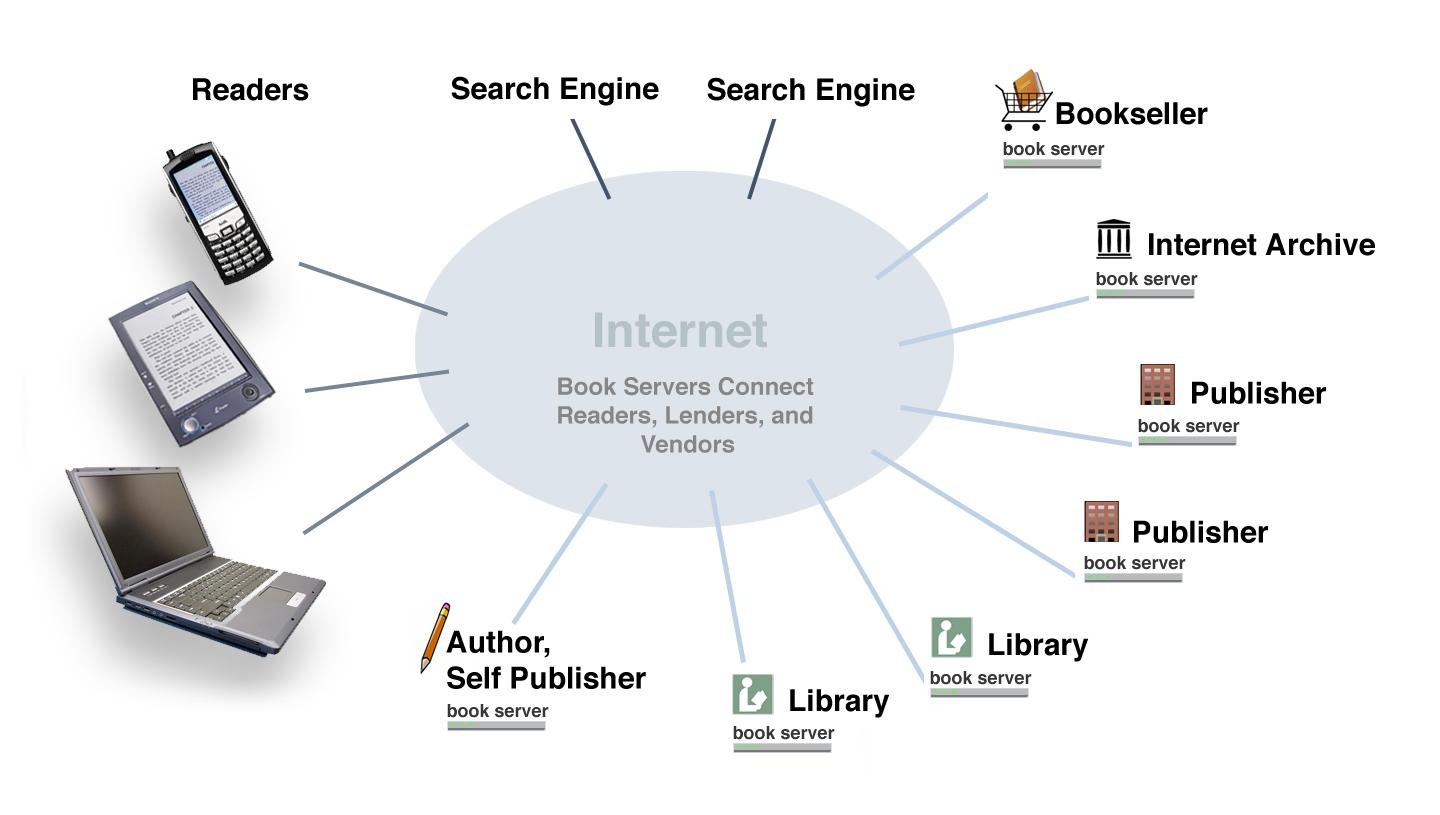
\includegraphics[scale=0.25]{web-of-books.png}

\subsection{نمایِ کارسازِ کتاب}
ساختِ معماریِ جدیدی که از استاندارهایِ بازی استفاده می‌کند که به مردم اجازه می‌دهد تا کتاب‌ها را از هر منبع، بر رویِ هر بستری، با استفاده از برنامه‌هایِ کاربردیِ کتاب‌هایِ دیجیتالیِ بسیار متنوع، پیدا، خرید، دریافت و بخوانند. در حقیقت کارسازِ کتاب یک زبانِ مشترک برایِ ارتباط بین ناشران، کتابخانه‌ها، کتابفروشی‌ها و کاربران تعریف می‌کند تا همگی با چنین زبانی با یکدیگر به تبادلِ اطلاعات بپردازند. در این حالت تمامیِ ناشرانِ دیجیتالی کتاب‌هایِ خود را بر اساسِ چنین مشخصه‌ای کاتالوگ می‌کنند که به نوعی کاتالوگ‌های کتابخانه‌ها توزیع (کتابخانه‌هایِ توزیع‌شده) می‌شوند.
\subsection{کارسازِ کتاب در عمل}
ناشرانِ محتوایی کاتالوگ می‌سازند.\\
سپس ...\\
\begin{enumerate}
	\item خوانندگان، کاتالوگِ عنوان‌هایِ کتاب را مرور می‌کنند ...
	\item عنوانِ کتابی را در نظر می‌گیرند ...
	\item کتاب را تهیه می‌کنند (پرداختِ وجه اگر نیاز باشد) ...
	\item آن را در قفسهٔ کتابِ کاربر قرار می‌دهد.
\end{enumerate}
در حقیقت کارسازِ کتاب، عملیاتِ پیچیدهٔ جست-و-جو، بررسی، تهیه، و دریافتِ کتاب را برایِ کاربر آسان می‌کند و مشکلاتی را که در قسمتِ طرحِ مشکل نام بردیم را از میان می‌برد.

\subsection{انرژیِ اتمی}
کاتالوگ‌هایِ کارسازِ کتاب، مبتنی بر استانداردِ عمومیِ اکس‌ام‌الی به نام اتم هستند، آن‌ها مفهومِ خوراک‌ها و وارده‌ها را که در قالبِ هم‌نشریِ اتم تعریف شده است، وام گرفته‌اند. اتم قالبِ مستندِ مبتنی-بر-اکس‌ام‌الی‌ست که فهرست‌هایِ مرتبطِ اطلاعاتی‌ست که با نامِ «خوراک» شناخته می‌شود. خوراک‌ها ترکیبی از اقلام، مشهور به «وارده‌ها»، است که هر کدام همراهِ مجموعه‌ٔ قابلِ گسترشِ فراداده‌هایِ پیوست‌شده است. برایِ مثال، هر وارده، نامی دارد. در اصل، خوراک، محفظه‌ای برایِ وارده‌ها است و همچنین هنگامِ مصرفِ اتم، ممکن است با یک فید یا یک واردهٔ منفرد برخورد کنید.
\subsection{خوراک‌هایِ ناوبری و خوراک‌هایِ دستیابی}
در کاتالوگِ اُپی‌دی‌اس، ما دو استفادهٔ متفاوت برایِ خوراک‌ها تعریف می‌کنیم:
\begin{enumerate}
	\item خوراک‌هایِ ناوبری، که توسطِ کارخواه برایِ مرور در کاتالوگ‌ها استفاده می‌شود.
	\item خوراک‌هایِ دستیابی، که نشریات فهرست می‌شوند و می‌توان آن‌ها را دریافت کرد.
\end{enumerate}
هر دو نوع کاتالوگ اتم‌هایِ معتبری هستند و می‌توانند توسطِ کارخواهِ اتمیِ عمومی مصرف شوند. از تولیدکنندگانِ کاتالوگ انتظار می‌رود که بینِ خوراک‌هایِ ناوبری و دستیابی تمایز قائل شوند: یک خوراک نمی‌تواند همزمان از هر دو نوع باشد.
\subsection{نشریات و پیوندهایِ کاتالوگ}
به روشِ مشابه، وارده‌ها در اُپی‌دی‌اس می‌توانند:
\begin{enumerate}
	\item پیوندهایِ کاتالوگ، باشند که به دیگر خوراک‌ها اشاره کنند و در خوراک‌هایِ ناوبری استفاده شوند.
	\item نشریات، فراداده‌هایِ متنوعی را فهرست می‌کنند و پیوندِ دسترسی را در خوراک‌هایِ دسترسی فراهم می‌کنند.
\end{enumerate}
نشریات با وجودِ پیوندِ دسترسی شناخته می‌شوند. فقدانِ چنین پیوندی نشان‌دهندهٔ این است که وارده یک پیوندِ کاتالوگ است.

برنامه‌هایِ کاربردی می‌توانند برای خواندن آن‌ها، در میانِ بسترهایِ متفاوتی سریعاً نوشته شوند. جهانی در ماورایِ اپل، آمازون، گوگل.
\subsection{تحویلِ محتوا}
همچنین کاتالوگ‌هایِ کارسازِ کتاب می‌توانند:
\begin{enumerate}
	\item توسطِ هر مهیاکنندهٔ رسانه‌ای منتشر شوند (از قبیلِ ناشر یا کتابخانه)، یا
	\item در مجموعهٔ بزرگی توسط بسترهایی که خدمات و دسترسی‌ها را مسیر می‌کند، مجتمع شوند.
\end{enumerate}

\subsection{توزیعِ متحوا}
کاتالوگ‌ها حاویِ داده‌هایِ ساده‌ای هستند که کتاب‌ها و نشانگرهایِ آن‌ها به نشانیِ منابعِ داده‌ها را توصیف می‌کنند. بردارهایِ باصرفه‌ای برایِ ارائهٔ مانیفستِ محتوا تولید می‌کنند.

\subsection{کاتالوگ از طریقِ ای‌پی‌آی}
استفاده از استانداردها برایِ توصیفِ داده، می‌تواند برایِ پیوند دادنِِ ساده‌ترِ داده‌ها استفاده شود. این را «داده‌هایِ پیوندی» می‌نامند.
\begin{enumerate}
	\item نظرات و بررسی‌هایِ کتاب
	\item فهرست‌هایِ مطالعه
	\item حاشیه‌نویسی‌ها
\end{enumerate}

\subsection{قفسه‌کتاب‌ها}
فیدبوک در استفاده از کاتالوگ‌هایی که قفسه‌کتاب‌هایِ قابلِ حمل فروشنده-بی‌طرف
\LTRfootnote{vendor-neutral}
، پیشگام است.
\begin{enumerate}
	\item ادارهٔ کتاب‌ها از خرده‌فروش‌هایِ متعدد.
	\item پشتیبان از پرونده‌ها (محلی، دراپ‌باکس)
	\item اضافه کردن کتاب‌ها به شبکه‌هایِ اجتماعی
	\item به اشتراک گذاریِ آنچه می‌خوانید.
\end{enumerate}
\bibliography{test}



\end{document}
